% Latex header for doxygen 1.8.9.1
\documentclass[twoside]{book}

% Packages required by doxygen
\usepackage{fixltx2e}
\usepackage{calc}
\usepackage{doxygen}
\usepackage[export]{adjustbox} % also loads graphicx
\usepackage{graphicx}
\usepackage[utf8]{inputenc}
\usepackage{makeidx}
\usepackage{multicol}
\usepackage{multirow}
\PassOptionsToPackage{warn}{textcomp}
\usepackage{textcomp}
\usepackage[nointegrals]{wasysym}
\usepackage[table]{xcolor}

% Font selection
\usepackage[T1]{fontenc}
\usepackage[scaled=.90]{helvet}
\usepackage{courier}
\usepackage{amssymb}
\usepackage{sectsty}
\renewcommand{\familydefault}{\sfdefault}
\allsectionsfont{%
  \fontseries{bc}\selectfont%
  \color{darkgray}%
}
\renewcommand{\DoxyLabelFont}{%
  \fontseries{bc}\selectfont%
  \color{darkgray}%
}
\newcommand{\+}{\discretionary{\mbox{\scriptsize$\hookleftarrow$}}{}{}}

% Page & text layout
\usepackage{geometry}
\geometry{%
  a4paper,%
  top=2.5cm,%
  bottom=2.5cm,%
  left=2.5cm,%
  right=2.5cm%
}
\usepackage[T1]{fontenc}
\usepackage{titlesec, blindtext, color}
\definecolor{gray75}{gray}{0.75}
\newcommand{\hsp}{\hspace{20pt}}
\titleformat{\chapter}[hang]{\Huge\bfseries}{\thechapter\hsp\textcolor{gray75}{|}\hsp}{0pt}{\Huge\bfseries}
\tolerance=750
\hfuzz=15pt
\hbadness=750
\setlength{\emergencystretch}{15pt}
\setlength{\parindent}{0cm}
\setlength{\parskip}{0.2cm}
\makeatletter
\renewcommand{\paragraph}{%
  \@startsection{paragraph}{4}{0ex}{-1.0ex}{1.0ex}{%
    \normalfont\normalsize\bfseries\SS@parafont%
  }%
}
\renewcommand{\subparagraph}{%
  \@startsection{subparagraph}{5}{0ex}{-1.0ex}{1.0ex}{%
    \normalfont\normalsize\bfseries\SS@subparafont%
  }%
}
\makeatother

% Headers & footers
\usepackage{fancyhdr}
\pagestyle{fancyplain}
\fancyhead[LE]{\fancyplain{}{\bfseries\thepage}}
\fancyhead[CE]{\fancyplain{}{}}
\fancyhead[RE]{\fancyplain{}{\bfseries\leftmark}}
\fancyhead[LO]{\fancyplain{}{\bfseries\rightmark}}
\fancyhead[CO]{\fancyplain{}{}}
\fancyhead[RO]{\fancyplain{}{\bfseries\thepage}}
\fancyfoot[LE]{\fancyplain{}{}}
\fancyfoot[CE]{\fancyplain{}{}}
\fancyfoot[RE]{\fancyplain{}{\bfseries\scriptsize Generated by Yu Chen }}
\fancyfoot[LO]{\fancyplain{}{\bfseries\scriptsize Generated by Yu Chen }}
\fancyfoot[CO]{\fancyplain{}{}}
\fancyfoot[RO]{\fancyplain{}{}}
\renewcommand{\footrulewidth}{0.4pt}
\renewcommand{\chaptermark}[1]{%
  \markboth{#1}{}%
}
\renewcommand{\sectionmark}[1]{%
  \markright{\thesection\ #1}%
}

% Indices & bibliography
\usepackage{natbib}
\usepackage[titles]{tocloft}
\setcounter{tocdepth}{3}
\setcounter{secnumdepth}{5}
\makeindex

% Hyperlinks (required, but should be loaded last)
\usepackage{ifpdf}
\ifpdf
  \usepackage[pdftex,pagebackref=true]{hyperref}
\else
  \usepackage[ps2pdf,pagebackref=true]{hyperref}
\fi
\hypersetup{%
  colorlinks=true,%
  linkcolor=blue,%
  citecolor=blue,%
  unicode%
}

% Custom commands
\newcommand{\clearemptydoublepage}{%
  \newpage{\pagestyle{empty}\cleardoublepage}%
}


%===== C O N T E N T S =====

\usepackage[yyyymmdd,hhmmss]{datetime}

\begin{document}

% Titlepage & ToC
\hypersetup{pageanchor=false,
             bookmarks=true,
             bookmarksnumbered=true,
             pdfencoding=unicode
            }
\pagenumbering{roman}
\begin{titlepage}
\vspace*{7cm}
\begin{center}%
{\Huge Dual State Framework}\\
\vspace*{0.5cm}
{\Large Design Documentation}\\
\vspace*{1cm}
{\normalsize Yu Chen - C00151352}\\
\vspace*{0.2cm}
{\small \today\ \currenttime}\\
\end{center}
\end{titlepage}
\clearemptydoublepage
\tableofcontents
\clearemptydoublepage
\pagenumbering{arabic}
\hypersetup{pageanchor=true}

%--- Begin generated contents ---
\chapter{Introduction}
\label{_introduction}
\hypertarget{_introduction}{}
The document describes all functionalities estimated to be implemented for the project. It also shows what level of quality of the project should be achieved. Project plan and schedule are embedded in this document. \hypertarget{_introduction_IntroductionPurpose}{}\section{Purpose}\label{_introduction_IntroductionPurpose}
The main purpose of my project is to create a C++ framework for parallel computing. Parallel computing is the science and art of programming computers that can do more than one operation at once during the same cycle, simultaneously and concurrently. It performs often via having more than one processor. ~\newline
~\newline
Next, A benchmark program is required for profiling this framework. The program will be designed as a G\+U\+I application which shows the performance in different situations \hypertarget{_introduction_IntroductionPlan}{}\section{Plan}\label{_introduction_IntroductionPlan}
Dual State Framework will be developed by C++ under Mac Os X. Open\+M\+P or Intel T\+B\+B is used for implementing Parallel Computing. In addition, it will be compiled and debugged both on Microsoft Windows and Linux as well. This process will be done by Cmake. The A\+P\+I Documentation of this project will be created by Doxygen. ~\newline
~\newline
The simple benchmark program will be written by C++ with S\+F\+M\+L or S\+D\+L library. Git will be used for source control and version control. The project is now available in following link. ~\newline
~\newline
\href{https://github.com/kuyoonjo/DualStateFramework}{\tt https\+://github.\+com/kuyoonjo/\+Dual\+State\+Framework} \hypertarget{_introduction_IntroductionPotentialUsers}{}\section{Potential Users}\label{_introduction_IntroductionPotentialUsers}
Dual State Framework can have a variety of uses. Initially the project is concerned around computer games, but it can be used in broad kinds of software. The framework can be used in any program or game that runs parallel processes. Currently almost all of them meet that criteria. 
\chapter{Framwork Design}
\label{_framework_design}
\hypertarget{_framework_design}{}
\hypertarget{_framework_design_FrameworkDesignArchitectureDesign}{}\section{Architecture Design}\label{_framework_design_FrameworkDesignArchitectureDesign}
The goal of this project is to implement concurrency and parallel. In this framework, each Synchronized Object process simultaneously after Dual State Framework started. The process shows as follow\+: 
\begin{DoxyImageNoCaption}
  \mbox{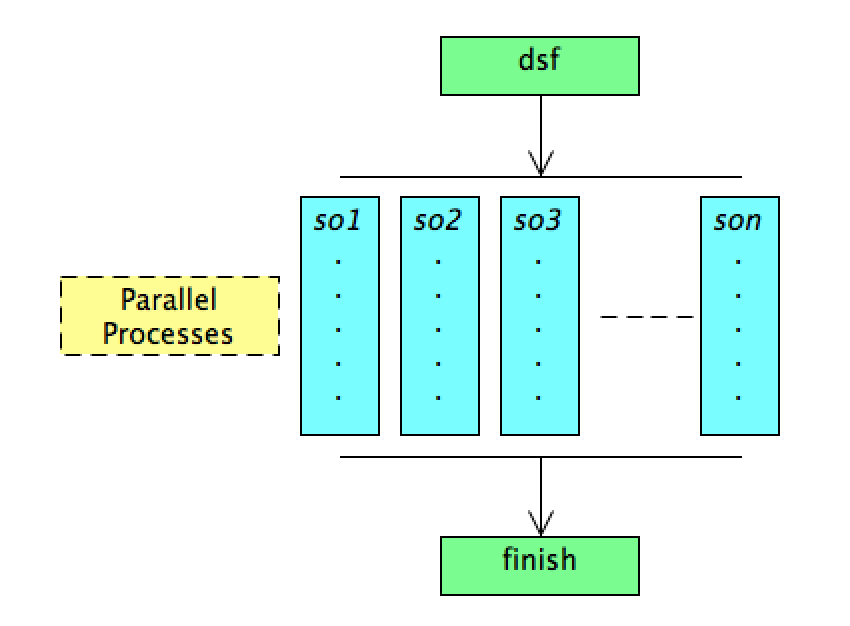
\includegraphics[width=\textwidth,height=\textheight/2,keepaspectratio=true]{DesignArchitecture.png}}
\end{DoxyImageNoCaption}

\begin{DoxyItemize}
\item \char`\"{}dsf\char`\"{} refers to Dual State Framework
\item \char`\"{}so\char`\"{} followed by a number refers to Synchronized Object
\end{DoxyItemize}\hypertarget{_framework_design_FrameworkDesignProceduralDesign}{}\section{Procedural Design}\label{_framework_design_FrameworkDesignProceduralDesign}
This diagram shows activities and interactions in one success evaluation(one frame in game). 
\begin{DoxyImageNoCaption}
  \mbox{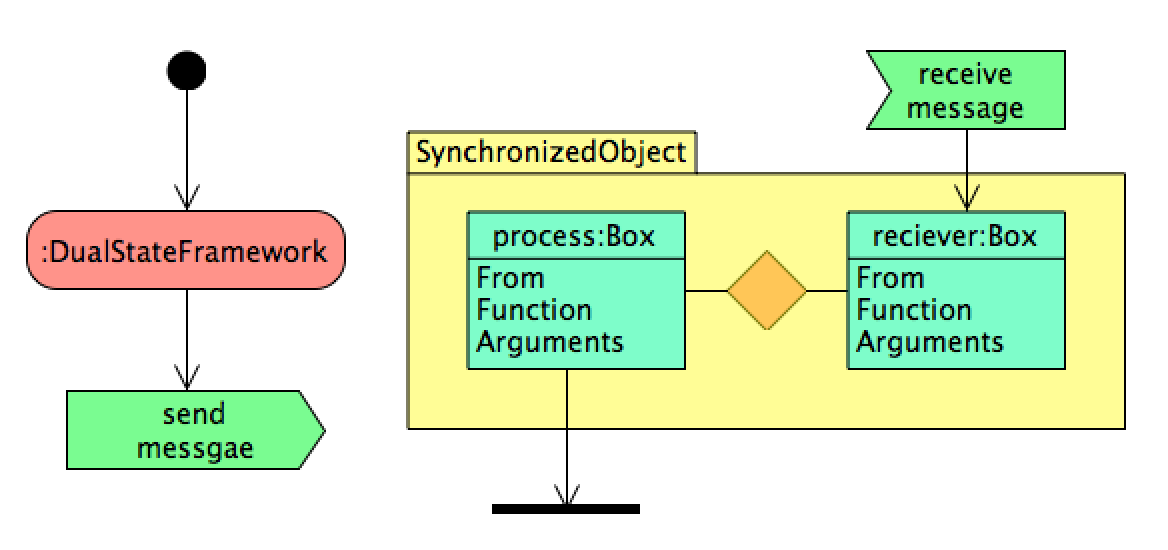
\includegraphics[width=\textwidth,height=\textheight/2,keepaspectratio=true]{DesignProcedure.png}}
\end{DoxyImageNoCaption}
 As it shows, the system create a Dual\+State\+Framework object. A Dual\+State\+Framework object can have many Synchronized\+Object objects. Each Synchronized\+Object object has two Boxes. One is for processing messages. The other one is for receiving messages. The sequence is like this\+:
\begin{DoxyEnumerate}
\item The Dual\+State\+Framework object starts with sending a “start” message.
\item Messages from receiver are popped out and then be pushed into processor.
\item Processor unpacks messages and evaluates function with arguments in each message sequently.
\end{DoxyEnumerate}

After step 3, it will go back to step 2. Step 2 and step 3 process alternatively and endlessly until the Dual\+State\+Framework object stopped.\hypertarget{_framework_design_FrameworkDesignInterfaceDesign}{}\section{Interface Design}\label{_framework_design_FrameworkDesignInterfaceDesign}
\hypertarget{_framework_design_FrameworkDesignInterfaceDesignNamespace}{}\subsection{Namespace}\label{_framework_design_FrameworkDesignInterfaceDesignNamespace}
All classes in this framework is under the namespace \char`\"{}dsf\char`\"{}, which is abbreviation of the project name \char`\"{}\+Dual State Framework\char`\"{}.\hypertarget{_framework_design_FrameworkDesignInterfaceDesigndsfRunnable}{}\subsection{dsf\+::\+Runnable}\label{_framework_design_FrameworkDesignInterfaceDesigndsfRunnable}
The interface provides a protected pure virtual function run(), which will be called when subclass object starts. For example\+: 
\begin{DoxyCode}
\textcolor{keyword}{class }MyDSF : \textcolor{keyword}{public} dsf::DualStateFrameword
\{
\textcolor{keyword}{protected}:
    \textcolor{keywordtype}{void} run()
    \{
        \textcolor{comment}{// do something here...}
    \}
\}

\textcolor{keywordtype}{void} main()
\{
    MyDSF dsf;
    dsf.start() \textcolor{comment}{// It will process MyDSF::run();}
\}
\end{DoxyCode}
\hypertarget{_framework_design_FrameworkDesignInterfacedsfDualStateFramework}{}\subsection{dsf\+::\+Dual\+State\+Framework}\label{_framework_design_FrameworkDesignInterfacedsfDualStateFramework}
The starting pointer for the framework is the abstract class dsf\+::\+Dual\+State\+Framework. It provides essential functions for associating and managing its components (Synchronized\+Object objects, function points, and etc.).\hypertarget{_framework_design_FrameworkDesignInterfacedsfSynchronisable}{}\subsection{dsf\+::\+Synchronisable}\label{_framework_design_FrameworkDesignInterfacedsfSynchronisable}
Class dsf\+::\+Synchronisable is a template interface. It has a template member variable “next” and a pure virtual function “synchronise”. The variable is a copy of current class. The function synchronises the current state. 
\begin{DoxyCode}
\textcolor{preprocessor}{#include <dsf/Synchronisable.h>}

\textcolor{keyword}{class }Vector3D
\{
\textcolor{keyword}{public}:
    \textcolor{keywordtype}{float} x, y, z;
    Vector3D(\textcolor{keywordtype}{float} x, \textcolor{keywordtype}{float} y, \textcolor{keywordtype}{float} z) : x(x), y(y), z(z)\{\}
\};

\textcolor{keyword}{class }SyncVector : \textcolor{keyword}{public} dsf::Synchronisable<Vector3D>, \textcolor{keyword}{public} Vector3D
\{
\textcolor{keyword}{public}:
    SyncInt(\textcolor{keywordtype}{float} x, \textcolor{keywordtype}{float} y, \textcolor{keywordtype}{float} z) : Vector3D(x, y, z) \{
        this->next = \textcolor{keyword}{new} Vector3D(x, y, z);
    \}
    \textcolor{keywordtype}{void} synchronise()\textcolor{keyword}{ override }\{
        this->x = this->next->x;
        this->y = this->next->y;
        this->z = this->next->z;
    \}
\};
\end{DoxyCode}
\hypertarget{_framework_design_FrameworkDesignInterfacedsfTaskBox}{}\subsection{dsf\+::\+Task\+Box}\label{_framework_design_FrameworkDesignInterfacedsfTaskBox}
The dsf\+::\+Task\+Box contains a list of dsf\+::\+Task objects. It provides essential methods to control the list such as “push”, “pop”, and “is\+Empty”.\hypertarget{_framework_design_FrameworkDesignInterfacedsfSynchronizedObject}{}\subsection{dsf\+::\+Synchronized\+Object}\label{_framework_design_FrameworkDesignInterfacedsfSynchronizedObject}
The dsf\+::\+Synchronized\+Object is a subclass of dsf\+::\+Task\+Box. In this framework, you can regard it as thread. It provides methods for implementing parallelism such as “send”, “receive”, and etc. Also, it implements interface dsf\+::\+Synchronisable$<$dsf\+::\+Task\+Box$>$. Therefore, it has two copies of dsf\+::\+Task\+Box. One is for receiving messages, and the other one is for executing messages. 
\begin{DoxyImageNoCaption}
  \mbox{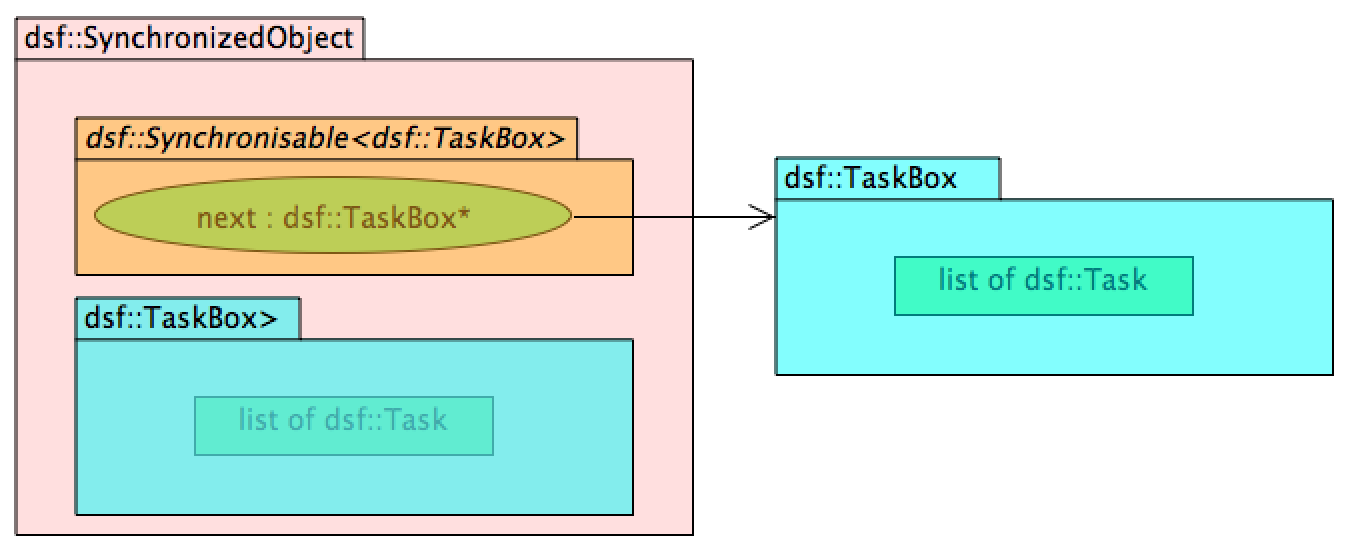
\includegraphics[width=\textwidth,height=\textheight/2,keepaspectratio=true]{DesignInterfaceSynchronizedObject.png}}
\end{DoxyImageNoCaption}
\hypertarget{_framework_design_FrameworkDesignInterfacedsfTask}{}\subsection{dsf\+::\+Task}\label{_framework_design_FrameworkDesignInterfacedsfTask}
This class have three members\+: from, function, and arguments, where \char`\"{}from\char`\"{} is a dsf\+::\+Synchronized\+Object object who sent message to you.\hypertarget{_framework_design_FrameworkDesignInterfacedsfArgument}{}\subsection{dsf\+::\+Argument}\label{_framework_design_FrameworkDesignInterfacedsfArgument}
A dsf\+::\+Argument object can refer to any type of object. The following code is allowed\+: 
\begin{DoxyCode}
dsf::Argument i = int(10);
dsf::Argument str = std::string(\textcolor{stringliteral}{"Hello"});
\end{DoxyCode}
\hypertarget{_framework_design_FrameworkDesignInterfacedsfTaskFunction}{}\subsection{dsf\+::\+Task\+Function}\label{_framework_design_FrameworkDesignInterfacedsfTaskFunction}
The message in a dsf\+::\+Task is an object of dsf\+::\+Task\+Function. An object of dsf\+::\+Task\+Function is a function pointer whose function takes two dsf\+::\+Synchronized\+Object objects, a dsf\+::\+Argument object as arguments. The constructor of dsf\+::\+Task\+Function takes a function pointer or a lambda expression as arguments. This is an example that uses lambda expression. 
\begin{DoxyCode}
dsf::TaskFunction* print = \textcolor{keyword}{new} dsf::TaskFunction([\textcolor{keyword}{this}](dsf::SynchronizedObject* to, 
                                                        dsf::SynchronizedObject* from,
                                                        dsf::TaskArgument* args)
                                                \{
                                                    \textcolor{keyword}{auto} syncObj = args->to<SyncObj*>();
                                                    std::cout << syncObj->getValue();
                                                    this->dsf->remove(to);
                                                \});
\end{DoxyCode}
\hypertarget{_framework_design_FrameworkDesignInterfacedsfSynchronizedVar}{}\subsection{dsf\+::\+Synchronized\+Var}\label{_framework_design_FrameworkDesignInterfacedsfSynchronizedVar}
The purpose of this class is to make thread-\/safe variables for dsf\+::\+Synchronized\+Object objects. A dsf\+::\+Synchronized\+Var object has two member variables -\/ “value” and “next”. The “value” is for read operation, and the “next” is for write operation. The function “synchronize” signs “next” to “value”. see example below\+: 
\begin{DoxyCode}
dsf::SynchronizedVar myInt; 
myInt = int(8); \textcolor{comment}{// value == NULL, next == 8}
myInt.synchronise(); \textcolor{comment}{// value == 8, next == 8}
std::cout << myInt.to<\textcolor{keywordtype}{int}>() << std::endl; \textcolor{comment}{// output 8}
myInt = int(9); \textcolor{comment}{// value == 8, next == 9}
std::cout << myInt.to<\textcolor{keywordtype}{int}>() << std::endl; \textcolor{comment}{// output 8}
myInt.synchronise(); \textcolor{comment}{// value == 9, next == 9}
std::cout << myInt.to<\textcolor{keywordtype}{int}>() << std::endl; \textcolor{comment}{// output 9}
\end{DoxyCode}
 
\begin{DoxyImageNoCaption}
  \mbox{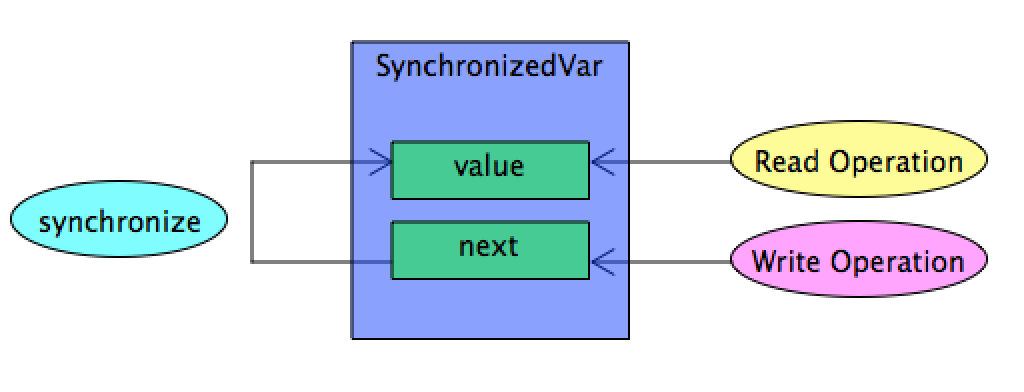
\includegraphics[width=\textwidth,height=\textheight/2,keepaspectratio=true]{DesignInterfaceSynchronizedVar.png}}
\end{DoxyImageNoCaption}
 
\chapter{Benchmark Program Design}
\label{_benchmark_program_design}
\hypertarget{_benchmark_program_design}{}
\hypertarget{_benchmark_program_design_BenchmarkProgramDesignGUIFramework}{}\section{G\+U\+I Framework}\label{_benchmark_program_design_BenchmarkProgramDesignGUIFramework}
To benchmark the framework, I will use S\+F\+M\+L to create a graphics application. When running the application, each frame runs many objects. The maximum, minimun, and average F\+P\+S(\+Frame per Second) is what I need for the benchmark. The application allows using different number of threads to run it.\hypertarget{_benchmark_program_design_BenchmarkProgramDesignGUIConfiguration}{}\section{G\+U\+I Configuration}\label{_benchmark_program_design_BenchmarkProgramDesignGUIConfiguration}
When you start the application, it will show you a configuration form like this\+: 
\begin{DoxyImageNoCaption}
  \mbox{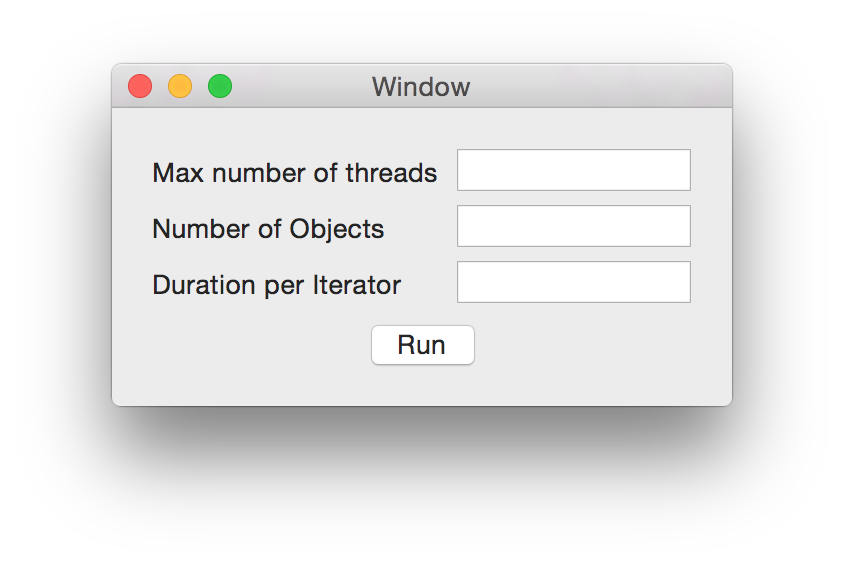
\includegraphics[width=\textwidth,height=\textheight/2,keepaspectratio=true]{DesignBenchmarkProgramDesignGUIConfiguration.png}}
\end{DoxyImageNoCaption}
 The application will run by using one thread to the max number of threads that user configured. The maximun, minimun, and average F\+P\+S will be recorded each iterator. Number of objects and duration for each iterator can be configured by this form.\hypertarget{_benchmark_program_design_BenchmarkProgramDesignOutputs}{}\section{Outputs}\label{_benchmark_program_design_BenchmarkProgramDesignOutputs}
The output is a bar graph which shows all information of the benchmark.
\begin{DoxyItemize}
\item x axis representing number of threads
\item y axis representing frames per second(\+F\+P\+S)
\item values with the maximum, the minimum, and the average.
\end{DoxyItemize}


\begin{DoxyImageNoCaption}
  \mbox{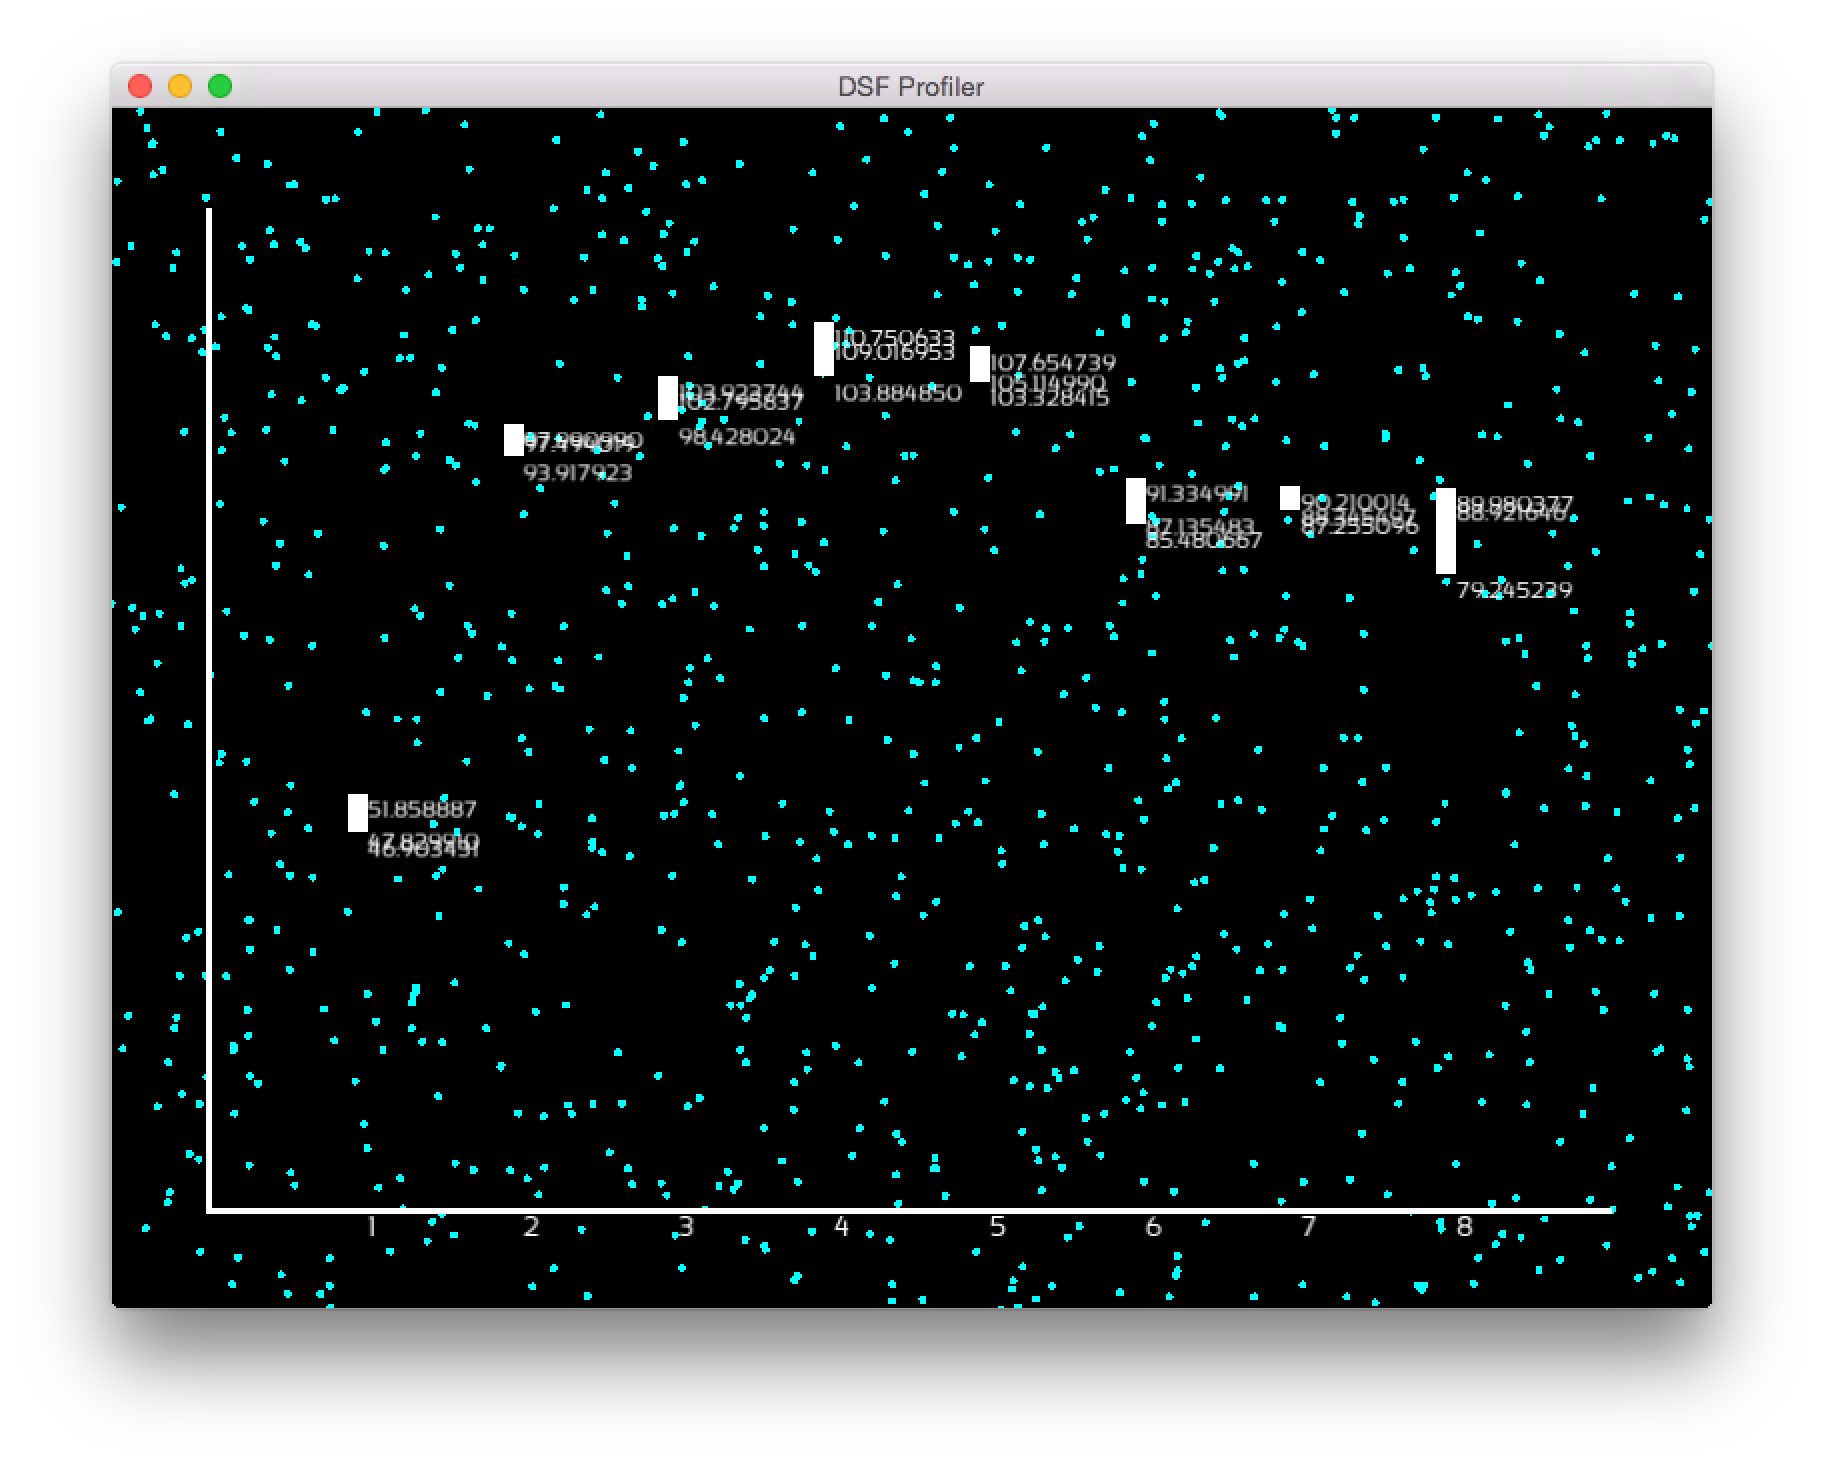
\includegraphics[width=\textwidth,height=\textheight/2,keepaspectratio=true]{DesignBenchmarkOutputs.png}}
\end{DoxyImageNoCaption}
 
%--- End generated contents ---

% Index
\backmatter
\newpage
\phantomsection
\clearemptydoublepage
\addcontentsline{toc}{chapter}{Index}
\printindex

\end{document}
